\documentclass[12pt]{article}

%\usepackage[top=4cm, bottom=4cm, left=4cm, right=4cm]{geometry}
%\usepackage{2in1}
%\usepackage{a4wide}
%\setlength{\columnsep}{1cm}

%\newcommand{\todo}[1]{{\bf \Huge !!!!! #1 !!!!!}}
\usepackage[textsize=footnotesize]{todonotes}
%\usepackage[british]{babel}
\usepackage[utf8]{inputenc}
\usepackage{url}
\usepackage{graphicx}
\usepackage{amssymb}
\usepackage{amsmath}
\usepackage{amsthm}
\usepackage{setspace}
\onehalfspacing
\usepackage{framed}
%\usepackage[usenames,dvipsnames]{color}
\usepackage[titles]{tocloft}
\setlength{\cftbeforesecskip}{0.1ex}
\renewcommand{\cftsecfont}{\rm}
\renewcommand{\cftsubsecfont}{\rm}
\renewcommand{\cftdot}{\ensuremath{\dots}}
\renewcommand{\cftsecdotsep}{3}
\renewcommand{\cftsubsecdotsep}{3}
\renewcommand{\cftsecpagefont}{\sl}
\renewcommand{\cftsubsecpagefont}{\sl}
\usepackage{sectsty}
\sectionfont{\large\it\centering}
\subsectionfont{\normalsize\it\centering}
\usepackage{listings}
%\usepackage{natbib}
\usepackage{fancyvrb}
\usepackage[margin=2cm]{geometry}
\usepackage[titletoc]{appendix}
\usepackage{bcprules}
\usepackage{tikz}
\usepackage{pgf}
\usetikzlibrary{arrows,automata}
\usepackage{tikz-cd}
\usetikzlibrary{positioning}
% boxes around figs
\usepackage{float}
\floatstyle{boxed} 
\restylefloat{figure}


\DefineVerbatimEnvironment{code}{Verbatim}{fontsize=\footnotesize}

\lstset{basicstyle=\tt\footnotesize}

\lstdefinelanguage{Haskell}
	{
		morekeywords={as, case, of, class, data, data, family, data, instance,
		default, deriving, do, forall, foreign, hiding, if, then, else, import,
		infix, infixl, infixr, let, in, mdo, module, newtype, proc, qualified,
		rec, type, where},
    	morecomment=[l]{--},
    	morecomment=[s]{{\{-}{-\}}},
    	morestring=[b]",
    	keywordstyle=\color{blue}\bf,
    	commentstyle=\it\color{ForestGreen},
    	stringstyle=\color{red},
    	literate= {<-}{{$\leftarrow$}}1 {->}{{$\rightarrow$}}1 {-<}{{$\prec$}}1
    	{=>}{{$\Rightarrow$}}1 {>>>}{{$\ggg$}}2 {<<<}{{$\lll$}}2 {***}{{$\times$}}1
    	{&&&}{{$\otimes$}}1  {'a}{{$\alpha$}}1 {'b}{{$\beta$}}1 {'c}{{$\gamma$}}1
    	{'d}{{$\delta$}}1 {'e}{{$\eta$}}1
    }

\newtheoremstyle{example}{\topsep}{\topsep}
     {\normalsize\sl} % Body font.
     {}               % Indent amount (empty = no indent, \parindent = para indent).
     {\small\it}      % Thm head font.
     {:}              % Punctuation after thm head.
     {\newline}       % Space after thm head (\newline = linebreak).
     {\thmname{#1} \thmnumber{#2}\thmnote{#3}} % Thm head spec.
\theoremstyle{example}
\newtheorem{example}{Example}

\newcommand{\hlinepage}{\rule{\textwidth}{0.25pt}}
\newcommand{\HRule}{\rule{\linewidth}{0.25pt}}
\newcommand{\fixme}[1]{\emph{\color{Red}\{!~#1~!\}}}

\begin{document}

\thispagestyle{empty}

\begin{center}

The National Institute of Aerospace / Galois Inc. / NASA LaRC

\vspace{0.1cm}

\HRule

\vspace{0.6cm}

{\Huge \bfseries
An Introduction to Copilot
}
\HRule

\vspace{0.6cm}

\begin{minipage}{0.4\textwidth}
\large
\begin{center}
Nis N. Wegmann\\
\small{
niswegmann@gmail.com\\
}

\end{center}
\end{minipage}
\begin{minipage}{0.4\textwidth}
\large
\begin{center}
Lee Pike\\
\small{
leepike@galois.com\\
}
\end{center}
\end{minipage}
\vspace{1cm}



\begin{minipage}{0.3\textwidth}
\large
\begin{center}
Chris Hathhorn \\
\small{
hathhorn@gmail.com\\
}
\end{center}
\end{minipage}
\begin{minipage}{0.3\textwidth}
\large
\begin{center}
Sebastian Niller\\
\small{
sebastian.niller@gmail.com\\
}
\end{center}
\end{minipage}

\vspace{1cm}

\begin{minipage}{0.3\textwidth}
\large
\begin{center}
Lauren Pick\\
\small{
lmpick@zoho.com\\
}
\end{center}
\end{minipage}
\begin{minipage}{0.3\textwidth}
\large
\begin{center}
Georges-Axel Jaloyan \\
\small{
georges-axel.jaloyan@ens.fr\\
}
\end{center}
\end{minipage}

\vspace{1cm}

{\large
Hampton, Virginia, United States, \today
}

%\begin{tabular}{cc}
%\hspace{0.5cm}\includegraphics[width=0.18\textwidth]{figures/nia}\hspace{0.5cm}  &
%\hspace{0.5cm}\includegraphics[width=0.2\textwidth]{figures/galois}\hspace{0.5cm} &
%\hspace{0.5cm}\includegraphics[width=0.2\textwidth]{figures/nasa}\hspace{0.5cm} \\
%\textsc{\large NIA} &
%\textsc{\large Galois Inc.} &
%\textsc{\large NASA LaRC} \\
%\end{tabular}

\let\thefootnote\relax\footnotetext{
This research is supported by NASA Contract NNL08AD13T from the Aviation Safety
Program Office.
}

\end{center}

\vspace{0.25cm}

\section*{Abstract}

{
\small
This document contains a tutorial on Copilot and its accompanying tools.
We do not attempt to give a complete, formal description of Copilot
(references are provided in the bibliography), rather we aim at
demonstrating the fundamental concepts of the language by using idiomatic
expositions and examples.
}

{
\small
\setcounter{tocdepth}{2}
\tableofcontents
}

\newpage
\addcontentsline{toc}{section}{Acknowledgement}
\section*{Acknowledgement}

The authors are grateful for NASA Contract NNL08AD13T to Galois Inc. and the
National Institute of Aerospace, which partially supported this work.
Thanks to Lars Kuhtz, Benedetto Di~Vito,  Robin Morisset, Kaveh
Darafsheh, Alwyn Goodloe.  

{




\section{Preliminaries}
\label{sec:preliminaries}

Copilot is embedded into the functional programming language Haskell
\cite{PeytonJones02}.  A working knowledge of Haskell is necessary to use
Copilot effectively; a variety of books and free web resources introduce Haskell.
Copilot uses Haskell language extensions
specific to the Glasgow Haskell Compiler (GHC); hence in order to start
using Copilot, you must first install an up-to-date version of GHC.
(The minimal required version is 7.10.1)
The easiest way to do this is to download and install the Haskell Platform,
which is freely distributed from here:

\begin{center}
\url{http://hackage.haskell.org/platform}
\end{center}

\noindent After having installed the Haskell Platform, Copilot is downloaded and
installed by executing the following command:

\begin{code}
> cabal install copilot
\end{code}

\noindent This should, if everything goes well, install Copilot on your system.

Copilot is distributed throughout a series of packages at Hackage:

\begin{itemize}
\item copilot-language: Contains the language front-end.
\item copilot-core: Contains an intermediate representation for Copilot programs (shared by all back-ends).
\item copilot-c99: A back-end for Copilot targeting C99 (based on Atom, \url{http://hackage.haskell.org/package/atom}). \textbf{Not updated anymore, might be deprecated soon.}
\item copilot-sbv: A back-end for Copilot targeting C99 (based on SBV, \url{http://hackage.haskell.org/package/sbv}).
\item copilot-libraries: A set of utility functions for Copilot, including a clock-library, a linear temporal logic framework,
a voting library, and a regular expression framework.
\item copilot-cbmc: A driver for proving the correspondence between code
  generated by the copilot-c99 and copilot-sbv back-ends.
\end{itemize}

Many of the examples in this paper can be found at
\url{https://github.com/Copilot-Language/Copilot/tree/copilot2.0/Examples}.
\todo[inline]{Update the version of Copilot when released (3.0 ?), and do not forget to put some examplesForACSL not already in the directory (WCV, TCAS, Self-Separation).}

To use the language, your Haskell module should contain the following import:
%
\begin{code}
import Language.Copilot  
\end{code}
%
To use the back-ends, import, them, respectively:
%
\begin{code}
import Copilot.Compile.C99
import Copilot.Compile.SBV
\end{code}
%
If you need to use functions defined in the Prelude that are redefined by
Copilot (e.g., arithmetic operators), import the Prelude as qualified:
%
\begin{code}
import qualified Prelude as P  
\end{code}


\section{Domain}

Copilot is a domain-specific language tailored to programming \emph{runtime
monitors} for \emph{hard real-time}, \emph{distributed}, \emph{reactive systems}.
Briefly, a runtime monitor is program that runs concurrently with a target program
with the sole purpose of assuring that the target program behaves in accordance with a
pre-established specification. Copilot is a language for writing such specifications.

A reactive system is a system that responds continuously to its environment.
All data to and from a reactive system is communicated progressively during
execution. Reactive systems differ from transformational systems which transforms
data in a single pass and then terminate, as for example compilers and numerical
computation software.

A hard real-time system is a system that has a statically bounded execution time
and memmory usage.  Typically, hard real-time systems are used in
mission-critical software, such as avionics, medical equipment, and nuclear power
plants; hence, occasional dropouts in the response time or crashes are not
tolerated.

A distributed system is a system which is layered out on multiple pieces of hardware.
The distributed systems we consider are all synchronized, i.e., each component agree on
a shared global clock.


\section{Language}~\label{sec:language}

Copilot is embedded into the functional programming language Haskell
\cite{PeytonJones02}, and a working knowledge of Haskell is necessary to use
Copilot effectively. Copilot is a pure declarative language; i.e., expressions
are free of side-effects and are referentially transparent.  A program written
in Copilot, which from now on will be referred to as a \emph{specification}, has
a cyclic behavior, where each cycle consists of a fixed series of steps:

\begin{itemize}
\item Sample external variables and arrays.
\item Update internal variables.
\item Fire external triggers. (In case the specification is violated.)
\item Update observers (for debugging purpose).
\end{itemize}

\noindent We refer to a single cycle as an \emph{iteration} or a \emph{step}.

All transformation of data in Copilot is propagated through streams.
A stream is an infinite, ordered sequence of values which must conform to the same type.
E.g., we have the stream of Fibonacci numbers:

\begin{center}
$s_{fib} = \{0, 1, 1, 2, 3, 5, 8, 13, 21, \dots \}$
\end{center}

\noindent We denote the $n$th value of the stream $s$ as $s(n)$, and the first
value in a sequence $s$ as $s(0)$. For example, for $s_{fib}$ we have that $s_{fib}(0) = 0$,
$s_{fib}(1) = 1$, $s_{fib}(2) = 1$, and so forth.

Constants as well as arithmetic, boolean, and relational operators are
lifted to work pointwise on streams:

\noindent
%\begin{minipage}{0.3\textwidth}
\begin{lstlisting}[language = Copilot, frame = single]
x :: Stream Int32
x = 5 + 5

y :: Stream Int32
y = x * x

z :: Stream Bool
z = x == 10 && y < 200
\end{lstlisting}
%\end{minipage}


\noindent Here the streams {\tt x}, {\tt y}, and {\tt z} are simply
\emph{constant streams}:

\begin{center}
$\mathtt{x} \leadsto \{10, 10, 10, \dots \}$,
$\mathtt{y} \leadsto \{100, 100, 100,  \dots \}$,
$\mathtt{z} \leadsto \{\mbox{T},\; \mbox{T},\; \mbox{T},\; \dots \}$
\end{center}

Two types of \emph{temporal} operators are provided, one for delaying streams and one for
looking into the future of streams:
%
\begin{lstlisting}[language = Copilot, frame = single]
(++) :: [a] -> Stream a -> Stream a
drop :: Int -> Stream a -> Stream a
\end{lstlisting}
%
Here {\tt xs ++ s} prepends the list {\tt xs} at the front of the stream {\tt s}.
For example the stream {\tt w} defined as follows, given our previous definition
of {\tt x}:
%
\begin{lstlisting}[language = Copilot, frame = single]
w = [5,6,7] ++ x
\end{lstlisting}
%
evaluates to the sequence
$\mathtt{w} \leadsto \{5, 6, 7, 10, 10, 10, \dots\}$.
The expression {\tt drop k s} skips the first {\tt k} values of the stream {\tt
  s}, returning the remainder of the stream.
For example we can skip the first two values of {\tt w}:
%
\begin{lstlisting}[language = Copilot, frame = single]
u = drop 2 w
\end{lstlisting}
%
which yields the sequence
$\mathtt{u} \leadsto \{7, 10, 10, 10, \dots\}$.

\subsection{Streams as Lazy-Lists} \label{sec:stream}

A key design choice in Copilot is that streams should mimic \emph{lazy lists}.
In Haskell, the lazy-list of natural numbers can be programmed like this:
%
\begin{lstlisting}[language = Copilot, frame = single]
nats_ll :: [Int32]
nats_ll = [0] ++ zipWith (+) (repeat 1) nats_ll
\end{lstlisting}
%
As both constants and arithmetic operators are lifted to work pointwise on
streams in Copilot, there is no need for {\tt zipWith} and {\tt repeat} when
specifying the stream of natural numbers:
%
\begin{lstlisting}[language = Copilot, frame = single]
nats :: Stream Int32
nats = [0] ++ (1 + nats)
\end{lstlisting}
%
In the same manner, the lazy-list of Fibonacci numbers can be specified  in Haskell as follows:
%
\begin{lstlisting}[language = Copilot, frame = single]
fib_ll :: [Int32]
fib_ll = [1, 1] ++ zipWith (+) fib_ll (drop 1 fib_ll)
\end{lstlisting}
%
In Copilot we simply throw away {\tt zipWith}:
\begin{lstlisting}[language = Copilot, frame = single]
fib :: Stream Int32
fib = [1, 1] ++ (fib + drop 1 fib)
\end{lstlisting}

Copilot specifications must be \emph{causal}, informally meaning that
stream values cannot depend on future values.  For example, the following stream
definition is allowed:
%
\begin{lstlisting}[language = Copilot, frame = single]
f :: Stream Word64
f = [0,1,2] ++ f

g :: Stream Word64
g = drop 2 f
\end{lstlisting}
%

But if instead {\tt g} is defined as {\tt g = drop 4 f}, then the definition is
disallowed.  While an analogous stream is definable in a lazy language, we bar
it in Copilot, since it requires future values of {\tt f} to be
generated before producing values for {\tt g}.  This is not possible since
Copilot programs may take inputs in real-time from the environment (see
Section~\ref{sec:interacting}).


\subsection{Structs}
Structs require some special attentation in Copilot, as we cannot magically
import the definition of the struct in Copilot. In this section we discuss the
steps that need to be taken by following the code of \texttt{Struct.hs} in the
\texttt{Examples} directory of the Copilot distribution, or the repository
\footnote{\url{https://github.com/Copilot-Language/Copilot/blob/master/Examples/Struct.hs}}.

Let's assume that we have defined a 2d-vector type in our C code:
\begin{lstlisting}
struct vec {
	float x;
	float y;
};
\end{lstlisting}
For us to be able to use this vector inside Copilot, we need to follow a number
of steps:
\begin{enumerate}
  \item Enable \texttt{DataKinds} compiler extension.
  \item Define a datatype to mimic the C definition.
  \item Write an instance of the \texttt{Struct} class, containing a definition
  for the struct name and function to translate the fields to a heterogeneous
    list.
  \item Write an instance of the \texttt{Typed} class.
\end{enumerate}

\subsubsection*{Enabling compiler extensions}
First and foremost, we need to enable the \texttt{DataKinds} extension to GHC,
by putting:
\begin{lstlisting}[language=Copilot]
{-# LANGUAGE DataKinds #-}
\end{lstlisting}
at the top of our specification file. This allows us to define \emph{kinds},
which are the types of types. Our datatype needs to carry the names of the
fields in C as well. Using the \texttt{DataKinds} extension we are able to
write the names of the fields as part of our types.


\subsubsection*{Defining the datatype}
A suitable representation of structs in Haskell is provided by the
\emph{record-syntax}, this allows us to use named fields as part of the
datatype. For Copilot this is not enough though: we still need to define the
names of the fields in our C code. Therefore we introduce new \texttt{Field}
datatype, which takes two arguments: the name of field, and it's type. Now we
can mimic our vector struct in Copilot as follows:
\begin{lstlisting}[language=Copilot]
data Vec = Vec
  { x :: Field "x" Float
  , y :: Field "y" Float
  }
\end{lstlisting}
Here we created two fields, $x$ and $y$, each with their corresponding C names
and types. Note that the name inside Haskell and the C names do not necessarily
need to match, nor is it always possible to have them match. For type-safety,
inside Copilot we will typically only use the Haskell level names (i.e. the
unquoted ones). The C names are only used by Copilot internally.


\subsubsection*{Instance of \texttt{Struct}}
Our next task is to inform Copilot about our new type, therefore we need to
write and instance of the \texttt{Struct}-class. This class has the purpose of
defining the datatype as a struct, it provides the code generator of Copilot the
name of struct in C, and provides a function to translate the struct to a list
of values:
\begin{lstlisting}[language=Copilot]
instance Struct Vec where
  -- typename :: Vec -> String
  typename _ = "vec"  -- Name of the type in C

  -- Function to translate Vec to list of Value's, order should match struct.
  -- tovalues :: Vec -> [Value Vec]
  toValues v = [ Value Float (x v)
               , Value Float (y v)
               ]
\end{lstlisting}
Both definitions should be pretty self-explanatory. Note however that
\texttt{Value a} is a wrapper around the \texttt{Field} datatype to hide the
actual type of \texttt{Field}. It takes the type of the field, and the field
itself as its arguments. The elements in the list should be in the same order
as the fields in the struct.

Both \texttt{typename} and \texttt{toValues} have to be defined by the user,
but neither should ever be used by the user. Both functions are only used by
the code generator of Copilot.


\subsubsection*{Instance of \texttt{Typed}}
In Copilot, streams can only of types that are instances of the \texttt{Typed}
class. To be able to create streams of vectors, \texttt{Vec} needs to be an
instance of \texttt{Typed} as well. The class only provides a \texttt{typeOf}
function, returning the type:
\begin{lstlisting}[language=Copilot]
instance Typed Vec where
  typeOf = Struct (Vec (Field 0) (Field 0))
\end{lstlisting}
For \texttt{Vec} this means we need to return something of the \texttt{Vec}
type wrapped in the \texttt{Struct} constructor. In this case it does not
matter what the values of the fields are, we just need to return something of
the correct type.


\subsection{Functions on Streams} \label{sec:FnOnStreams}

Given that constants and operators work pointwise on streams, we can use Haskell
as a macro-language for defining functions on streams.  The idea of using
Haskell as a macro language is powerful since Haskell is a
general-purpose higher-order functional language.

\begin{example}
We define the function {\tt even}, which given a stream of
integers returns a boolean stream which is true whenever the input stream
contains an even number, as follows:
%
\begin{lstlisting}[language = Copilot, frame = single]
even :: Stream Int32 -> Stream Bool
even x = x `mod` 2 == 0
\end{lstlisting}
%
Applying {\tt even} on {\tt nats} (defined above) yields the sequence
$\{T, F, T, F, T, F, \dots\}$.
\end{example}

If a function is required to return multiple results, we simply use plain
Haskell tuples:

\begin{example}
We define complex multiplication as follows:
%
\begin{lstlisting}[language = Copilot, frame = single]
mul_comp
  :: (Stream Double, Stream Double)
  -> (Stream Double, Stream Double)
  -> (Stream Double, Stream Double)
(a, b) `mul_comp` (c, d) = (a * c - b * d, a * d + b * c)
\end{lstlisting}
%
Here {\tt a} and {\tt b} represent the real and imaginary part of the left
operand, and {\tt c} and {\tt d} represent the real and imaginary part
of the right operand.
\end{example}

\subsection{Stateful Functions} \label{sec:stateful}

In addition to pure functions, such as {\tt even} and {\tt mul\_comp},
Copilot also facilitates \emph{stateful} functions. A \emph{stateful} function
is a function which has an internal state, e.g. as a latch (as in electronic
circuits) or a low/high-pass filter (as in a DSP).

\begin{figure*}
\begin{minipage}{0.25\linewidth}
\begin{tabular}{c|c||c}
$\mathtt{x}_i$: & $\mathtt{y}_{i-1}$: & $\mathtt{y}_i$:\\
\hline
$F$ & $F$ & $F$ \\
\hline
$F$ & $T$ & $T$ \\
\hline
$T$ & $F$ & $T$ \\
\hline
$T$ & $T$ & $F$
\end{tabular}
\end{minipage}
\begin{minipage}{0.35\linewidth}
\begin{lstlisting}[frame=none]
latch :: Stream Bool -> Stream Bool
latch x = y
  where
  y = if x then not z else z
  z = [False] ++ y
\end{lstlisting}
\end{minipage}
\hspace{1cm}
\begin{minipage}{0.3\linewidth}
\begin{tabular}{c|c|c|c|c|c}
   & 0 & 1 & 2 & 3 & 4\\
\hline
x & $F$ & $T$ & $T$ & $F$ & $F$ \\
\hline
y & $F$ & $T$ & $F$ & $F$ & $F$ \\
\end{tabular}
\end{minipage}
\caption{A latch [Example 3]. The specification function is provided at the left and the
implementation in copilot is provided in the middle. The right shows an example of
the latch, where x is $\{F, T, T, F, F, \dots \}$ and the initial value of y (used with $x_0$ to find
$y_0$ since there is no $y_{-1}$) is False.}
\label{fig:jk_latch}
\end{figure*}

\begin{example}
We consider a simple latch, as described in \cite{Farhat2004}, with a single
input and a boolean state. A latch is a way of simulating memory in circuits by feeding
back output gates as inputs.  Whenever the input is true the internal state is reversed.
The operational behavior and the implementation of the latch is shown in Figure
\ref{fig:jk_latch}.\footnote
{In order
to use conditionals (i.e., if-then-else) in Copilot specifications,
as in Figures~\ref{fig:jk_latch} and~\ref{fig:counter}, the GHC
language extension {\tt RebindableSyntax} must be set on.}
\end{example}

\begin{figure*}
\begin{minipage}{0.4\linewidth}
\begin{tabular}{c|c||c}
$\mathtt{inc}_i$: & $\mathtt{reset}_i$: & $\mathtt{cnt}_i$: \\
\hline
$F$ & $F$ & $\mathtt{cnt}_{i-1}$ \\
\hline
* & $T$ & $0$ \\
\hline
$T$ & $F$ & $\mathtt{cnt}_{i-1} + 1$ \\
\hline
\end{tabular}
\end{minipage}
\hspace{1cm}
\begin{minipage}{0.6\linewidth}
\begin{lstlisting}[language = Copilot, frame = none]
counter :: Stream Bool -> Stream Bool
        -> Stream Int32
counter inc reset = cnt
  where
  cnt = if reset then 0
          else if inc then z + 1
                 else z
  z = [0] ++ cnt
\end{lstlisting}
\end{minipage}
\caption{A resettable counter. The specification is provided at the left and the
implementation is provided at the right.
}
\label{fig:counter}
\end{figure*}

\begin{example}
We consider a resettable counter with two inputs, {\tt inc} and {\tt reset}.
The input {\tt inc} increments the counter and the input {\tt reset} resets the
counter. The internal state of the counter, {\tt cnt}, represents the value of the
counter and is initially set to zero. At each cycle, $i$, the value of
$\mathtt{cnt}_i$ is determined as shown in the left table in Figure
\ref{fig:counter}.
\end{example}

%\begin{figure}
%\begin{code}
%fir2pole :: Double -> Double -> Double -> Double
%  -> Double -> Sig Double -> Sig Double
%fir2pole a1 a2 b0 b1 b2 x0 = y0
%  where
%    y0 = - (constant a1)*y1 - (constant a2)*y2
%         + (constant b0)*x0 + (constant b1)*x1 + (constant b2)*x2
%    x2 = [0, 0] ++ x0 ; x1 = drop 1 x2
%    y2 = [0, 0] ++ y0 ; y1 = drop 1 y2
%\end{code}
%\caption{A $2$-pole IIR filter.}
%\label{fig:2_pole_iir_filter}
%\end{figure}

\subsection{Types} \label{sec:types}

Copilot is a typed language, where types are enforced by the Haskell type system
to ensure generated C programs are well-typed.  Copilot is \emph{strongly typed}
(i.e., type-incorrect function application is not possible) and \emph{statically
  typed} (i.e., type-checking is done at compile-time).  The base types are
Booleans, unsigned and signed words of width 8, 16, 32, and 64, floats, and
doubles.  All elements of a stream must belong to the same base
type.  These types have instances for the class {\tt Typed a}, used to constrain
Copilot programs.

We provide a {\tt cast} operator
%
\begin{lstlisting}[language = Copilot, frame = single]
cast :: (Typed a, Typed b) => Stream a -> Stream b
\end{lstlisting}
%
that casts from one type to another.  The cast operator is only defined for
casts that do not lose information, so an unsigned word type {\tt a} can only be
cast to another unsigned  type at least as large as {\tt a} or to a signed word
type strictly larger than {\tt a}.  Signed types cannot be cast to unsigned
types but can be cast to signed types at least as large.

There also exists an {\tt unsafeCast} operator which allows casting from any
type to any other (except from floating point numbers to integer types):

\begin{lstlisting}[language = Copilot, frame = single]
unsafeCast :: (Typed a, Typed b) => Stream a -> Stream b
\end{lstlisting}

\subsection{Interacting With the Target Program}
\label{subsec:interacting}

All interaction with the outside world is done by sampling \emph{external
  symbols} and by evoking \emph{triggers}.  External symbols are symbols that
are defined outside Copilot and which reflect the visible state of the target
program that we are monitoring.  They include variables and arrays.
Analogously, triggers are functions that are defined outside Copilot and which
are evoked when Copilot needs to report that the target program has violated a
specification constraint.

\paragraph{External Variables.}


As discussed in Section~\ref{sampling}, \emph{sampling} is an approach
for monitoring the state of an executing system based on sampling
state-variables, while assuming synchrony between the monitor and the
observed software. Copilot targets hard real-time embedded C programs
so the state variables that are observed by the monitors are variables
of C programs. Copilot monitors run either in the same thread or a
separate thread as the system under observation and the only variables
that can be observed are those that are made available through shared
memory. This means local variables cannot be observed. Currently,
Copilot supports basic C datatypes, arrays and structs. Combinations of each of
those work as well: nested arrays, arrays of structs, structs containg arrays
etc. All of these variables containing actual data; pointers to data are not
supported by design.


Copilot has both an interpreter and a compiler.The compiler must be
used to monitor an executing program. The Copilot reification process
generates a C monitor from a Copilot specification. The variables that
are observed in the C code must be declared as \emph{external}
variables in the monitor. The external variables have the same name as
the variables being monitored in the C code are treated as shared
memory. The interpreter is intended for exploring ideas and algorithms
and is not intended to monitor executing  C
programs. It may seem external variables would have no meaning if the
monitor was run in the interpreter, but Copilot gives the user the
ability to specify default stream values for an external variable that
get used when the monitor interpreted.

 A Copilot specification is \emph{open} if defined with external symbols in the
sense that values must be provided externally at runtime.  To simplify writing
Copilot specifications that can be interpreted and tested, constructs for
external symbols take an optional environment for interpretation.

External variables are similar to global variables in other languages. They
are defined by using the {\tt extern} construct:
%
\begin{lstlisting}[language = Copilot, frame = single]
extern :: Typed a => String -> Maybe [a] -> Stream a
\end{lstlisting}
%
\noindent
It takes the name of an external variable, a possible Haskell list to serve as
the environment for the interpreter, and generates a stream by sampling the
variable at each clock cycle.  For example,
%
\begin{lstlisting}[language = Copilot, frame = single]
sumExterns :: Stream Word64
sumExterns = let ex1 = extern "e1" (Just [0..])
                 ex2 = extern "e2" Nothing
             in  ex1 + ex2
\end{lstlisting}
%
is a stream that takes two external variables {\tt e1} and {\tt e2} and adds
them.  The first external variable contains the infinite list {\tt [0,1,2,...]}
of values for use when interpreting a Copilot specification containing the
stream.  The other variable contains no environment ({\tt sumExterns} must have
an environment for both of its variables to be interpreted).

Sometimes, type inference cannot infer the type of an external variable.  For
example, in the stream definition
%
\begin{lstlisting}[language = Copilot, frame = single]
extEven :: Stream Bool
extEven = e0 `mod` 2 == 0
  where e0 = externW8 "x" Nothing
\end{lstlisting}
%
\noindent
the type of {\tt extern "x"} is ambiguous, since it cannot be inferred from a
Boolean stream and we have not given an explicit type signature.  For
convenience, typed {\tt extern} functions are provided, e.g., {\tt externW8} or
{\tt externI64} denoting an external unsigned 8-bit word or signed 64-bit word,
respectively.
% Please see the grammar in Appendix~\ref{sec:BNF} for the list of
% all sampling functions.

In general it is best practice to define external symbols with
top-level definitions, e.g.,
%
\begin{lstlisting}[language = Copilot, frame = single]
e0 :: Stream Word8
e0 = extern  "e0" (Just [2,4..])
\end{lstlisting}

\noindent
so that the symbol name and its environment can be shared between streams.

Just like regular variables, arrays can be sampled as well. Copilot threats
arrays in the same way as it does for scalars. 
\begin{example}
\label{exmp:pitot}
Lets take the example where we
have the readouts of four pitot tubes, giving us the measured airspeed:
\begin{code}[frame=single]
/* Array containing readouts of 4 pitot tubes. */
double airspeeds[4] = ... ;
\end{code}
In our Copilot specification, we need to provide the type of our array, because
Copilot need to know the length of the array we refer to. Apart from that,
referring to an external array is like referring to any other variable:
\begin{lstlisting}[language=Copilot, frame=single]
airspeeds :: Stream (Array 4 Double)
airspeeds = extern "airspeeds" Nothing
\end{lstlisting}
\end{example}


\paragraph{Triggers.}
Triggers, the only mechanism for Copilot streams to effect the outside world,
are defined by using the {\tt trigger construct}:
%
\begin{lstlisting}[language = Copilot, frame = single]
trigger :: String -> Stream Bool -> [TriggerArg] -> Spec
\end{lstlisting}
%
The first parameter is the name of the external function, the second parameter is the
guard which determines when the trigger should be evoked, and the third parameter
is a list of arguments which is passed to the trigger when evoked.
Triggers can be combined into a specification by using the \emph{do}-notation:
%
\begin{lstlisting}[language = Copilot, frame = single]
spec :: Spec
spec = do
  trigger "f" (even nats) [arg fib, arg (nats * nats)]
  trigger "g" (fib > 10) []
  let x = externW64 "x" (Just [1..])
  trigger "h" (x < 10) [arg x]
\end{lstlisting}
%
The order in which the triggers are defined is irrelevant. To interpret this spec we run:
%
\begin{lstlisting}[language = Copilot, frame = single]
interpret 10 spec
\end{lstlisting}
%
which will yield the following output:
%
\begin{code}
f:        g:	 h:
(1,0)     ()        (1)
--        ()        (2)
(2,4)     ()        (3)
--        ()        (4)
(5,16)    ()        (5)
--        ()        (6)
(13,36)   --	(7)
--        --        (8)
(34,64)   --	(9)
--        --         --
\end{code}
%

\begin{example}
\label{exm:engine}
We consider an engine controller with the following property: If the temperature
rises more than 2.3 degrees within 0.2 seconds, then the fuel injector should
not be running.  Assuming that the global sample rate is 0.1 seconds, we can
define a monitor that surveys the above property:
%
\begin{lstlisting}[language = Copilot, frame = single]
propTempRiseShutOff :: Spec
propTempRiseShutOff =
  trigger "over_temp_rise"
    (overTempRise && running) []

  where
  max = 500 -- maximum engine temperature

  temps :: Stream Float
  temps = [max, max, max] ++ temp

  temp = extern "temp" Nothing

  overTempRise :: Stream Bool
  overTempRise = drop 2 temps > (2.3 + temps)

  running :: Stream Bool
  running = extern "running" Nothing
\end{lstlisting}
%

Here, we assume that the external variable {\tt temp} denotes the temperature of
the engine and the external variable {\tt running} indicates whether the fuel
injector is running.  The external function {\tt over\_temp\_rise} is called
without any arguments if the temperature rises more than 2.3 degrees within 0.2
seconds and the engine is not shut off.  Notice there is a latency of one tick between when the property is violated and when the guard becomes true.
\end{example}

\section{Tools} \label{sec:tools}

Copilot comes with a variety of tools, including a pretty-printer, an interpreter,
two compilers targeting C, and a verifier front-end. In the following section, we will
demonstrate some of these tools and their usage.

\subsection{Pretty-Printing} \label{sec:pretty-printing}
Pretty-printing is straightforward.  For some specification {\tt spec},
%
\begin{code}
prettyPrint spec
\end{code}
%
\noindent
returns the specification after static macro expansion.  Pretty-printing can
provide some indication about the complexity of the specification to be
evaluated.  Specifications that are built by recursive Haskell programs (e.g.,
the majority voting example in Section~\ref{subsec:boyer_moore}) can generate
expressions that are large.  Large expressions can take significant
time to interpret or compile.


\subsection{Proofs of Monitors}~\label{sec:proof} 

\todo{Chris, please add an intro to using the Copilot Model Checking
  capabilities} 


\subsection{Interpreting Copilot}

The copilot interpreter is invoked as follows (e.g. within GHCI, the GHC compiler's
interpreter for Haskell):
%
\begin{code}
GHCI> interpret 10 propTempRiseShutOff
\end{code}
%
The first argument to the function \emph{interpret} is the number of iterations that we want to evaluate.
The third argument is the specification (of type {\tt Spec}) that we wish to interpret.

The interpreter outputs the values of the arguments passed to the trigger, if
its guard is true, and {\tt --} otherwise.  For example, consider the following
Copilot program:
%
\begin{code}
spec = do 
  trigger "trigger1" (even nats) [arg nats, arg $ odd nats]
  trigger "trigger2" (odd nats) [arg nats]
\end{code}
% $
where {\tt nats} is the stream of natural numbers, and {\tt even} and {\tt odd}
are functions that take a stream and return whether the point-wise values are
even or odd, respectively.  The output of 
%
\begin{code}
interpret 10 spec
\end{code}
%
is as follows:
%
\begin{code}
trigger:   trigger2: 
(0,false)  --        
--         (1)       
(2,false)  --        
--         (3)       
(4,false)  --        
--         (5)       
(6,false)  --        
--         (7)       
(8,false)  --        
--         (9)     
\end{code}
%

Sometimes it is convenient to observe the behavior of a stream without defining
a trigger.  We can do so declaring an \emph{observer}.  For example:
%
\begin{code}
spec :: Spec
spec = observer ``obs'' nats  
\end{code}
%
can be interpreted using
%
\begin{code}
interpret 5 spec  
\end{code}
%
as usual.  Observers can be combined in larger Copilot programs.  For example,
consider the following:
%
\begin{code}
spec :: Spec
spec = do
  let x = externW8 "x" (Just [0..])
  trigger "trigger" true [arg $ x < 3]
  observer "debug_x" x
\end{code}
% $
Interpreting {\tt spec} as follows
%
\begin{code}
interpret 10 spec
\end{code}
%
yields
%
\begin{code}
trigger:  debug_x: 
(true)    0        
(true)    1        
(true)    2        
(false)   3        
(false)   4        
(false)   5        
(false)   6        
(false)   7        
(false)   8        
(false)   9        
\end{code}

\subsection{Compiling Copilot}  \label{sec:compiling}

Compiling the engine controller from Example \ref{exm:engine} is
straightforward.  First, we pick a back-end to compile to.  Currently, two
back-ends are implemented, both of which generate constant-time and
constant-space C code.  One back-end is called \emph{copilot-c99} and targets
the Atom language,\footnote{\url{http://hackage.haskell.org/package/atom}}
originally developed by Tom Hawkins at Eaton Corp. for developing control
systems.  The second back-end is called \emph{copilot-sbv} and targets the SBV
language\footnote{\url{http://hackage.haskell.org/package/sbv}}, originally
developed by Levent Erk\"{o}k.  SBV is primarily used as an interface to SMT
solvers~\cite{smt} and also contains a C-code generator.  Both
languages are open-source.

The two back-ends are installed with Copilot, and they can be imported,
respectively, as

\begin{code}
import Copilot.Compile.C99
\end{code}
\noindent
and
\begin{code}
import Copilot.Compile.SBV
\end{code}

After importing a back-end, the interface for compiling is as
follows:\footnote{Two explanations are in order: (1) {\tt reify} allows sharing in the expressions to be compiled~\cite{DSLExtract}, and {\tt >>=} is a higher-order
  operator that takes the result of reification and ``feeds'' it to the compile
  function.}
%
\begin{code}
reify spec >>= compile defaultParams
\end{code}
%
\noindent
(The compile function takes a parameter to rename the generated C files; {\tt
  defaultParams} is the default, in which there is no renaming.)

The compiler now generates two files:

\begin{itemize}
\item ``copilot.c'' --- 
\item ``copilot.h'' --- 
\end{itemize}

The file named ``copilot.h'' contains prototypes for all external variables, functions, and arrays,
and contains a prototype for the ``step''-functions which evaluates a single iteration.

\begin{code}
/* Generated by Copilot Core v. 0.1 */

#include <stdint.h>
#include <stdbool.h>

/* Triggers (must be defined by user): */

void over_temp_rise();

/* External variables (must be defined by user): */

extern float temp;
extern bool running;

/* Step function: */

void step();
\end{code}

Using the prototypes in ``copilot.h'' we can build a driver as follows:

\begin{code}
/* driver.c */
#include <stdio.h>
#include "copilot.h"

bool running = true;
float temp = 1.1;

void over_temp_rise()
{
  printf("The trigger has been evoked!\n");
}

int main (int argc, char const *argv[])
{
  int i;

  for (i = 0; i < 10; i++)
  {
    printf("iteration: %d\n", i);
    temp = temp * 1.3;
    step();
  }

  return 0;
}
\end{code}

Running ``gcc copilot.c driver.c -o prop'' gives a program ``prop'', which when executed
yields the following output:
%
\begin{code}
iteration: 0
iteration: 1
iteration: 2
iteration: 3
iteration: 4
iteration: 5
iteration: 6
iteration: 7
The trigger has been evoked!
iteration: 8
The trigger has been evoked!
iteration: 9
The trigger has been evoked!
\end{code}
%

\subsection{Correcness of the generated code}

\todo{George-Axel} describe what must be done to invoke the provers. 
 
\section{Extended Example: The Boyer-Moore Majority-Vote Algorithm}
\label{subsec:boyer_moore}

In this section we demonstrate how to use Haskell as an advanced macro language
on top of Copilot by implementing an algorithm for solving the voting problem
in Copilot.

\begin{figure*}[!htb]
\begin{lstlisting}[language = Copilot, frame = none]
majorityPure :: Eq a => [a] -> a
majorityPure []     = error "majorityPure: empty list!"
majorityPure (x:xs) = majorityPure' xs x 1

majorityPure' []     can _   = can
majorityPure' (x:xs) can cnt =
  let
    can' = if cnt == 0 then x else can
    cnt' = if cnt == 0 || x == can then succ cnt else pred cnt
  in
    majorityPure' xs can' cnt'
\end{lstlisting}
\caption{The first pass of the majority vote algorithm in Haskell.}
\label{fig:majority_pure}
\end{figure*}

\begin{figure*}[!htb]
\begin{lstlisting}[language = Copilot, frame = none]
aMajorityPure :: Eq a => [a] -> a -> Bool
aMajorityPure xs can = aMajorityPure' 0 xs can > length xs `div` 2

aMajorityPure' cnt []     _   = cnt
aMajorityPure' cnt (x:xs) can =
  let
    cnt' = if x == can then cnt+1 else cnt
  in
    aMajorityPure' cnt' xs can
\end{lstlisting}
\caption{The second pass of the majority vote algorithm in Haskell.}
\label{fig:amajority_pure}
\end{figure*}

Reliability in mission critical software is often improved by replicating
the same computations on separate hardware and by doing a vote in the end
based on the output of each system. The majority vote problem consists of
determining if in a given list of votes there is a candidate that has more
than half of the votes, and if so, of finding this candidate.

The Boyer-Moore Majority Vote Algorithm \cite{MooreBoyer82,Hesselink2005} solves
the problem in linear time and constant memory. It does so in two passes: The
first pass chooses a candidate; and the second pass asserts that the
found candidate indeed holds a majority.

Without going into details of the algorithm, the first pass can be implemented
in Haskell as shown in Figure \ref{fig:majority_pure}. The second pass, which
simply checks that a candidate has more than half of the votes, is
straightforward to implement and is shown in Figure \ref{fig:amajority_pure}.
E.g. applying {\tt majorityPure} on the string {\tt AAACCBBCCCBCC} yields {\tt
  C}, which {\tt aMajorityPure} can confirm is in fact a majority.

\begin{figure*}[!htb]
\begin{lstlisting}[language = Copilot, frame = none]
majority :: (Eq a, Typed a) => [Stream a] -> Stream a
majority []     = error "majority: empty list!"
majority (x:xs) = majority' xs x 1

majority' []     can _   = can
majority' (x:xs) can cnt =
  local
    (if cnt == 0 then x else can) $
      \ can' ->
        local (if cnt == 0 || x == can then cnt+1 else cnt-1) $
          \ cnt' ->
            majority' xs can' cnt'
\end{lstlisting}
\caption{The first pass of the majority vote algorithm in Copilot.}
\label{fig:majority}
\end{figure*}

\begin{figure*}[!htb]
\begin{lstlisting}[language = Copilot, frame = none]
aMajority :: (Eq a, Typed a) => [Stream a] -> Stream a -> Stream Bool
aMajority xs can = aMajority' 0 xs can > (fromIntegral (length xs) `div` 2)

aMajority' cnt []     _   = cnt
aMajority' cnt (x:xs) can =
  local
    (if x == can then cnt+1 else cnt) $
      \ cnt' ->
        aMajority' cnt' xs can
\end{lstlisting}
\caption{The second pass of the majority vote algorithm in Copilot.}
\label{fig:amajority}
\end{figure*}
% $

When implementing the majority vote algorithm for Copilot, we can use reuse
almost all of the code from the Haskell implementation. However, as functions
in Copilot are macros that are expanded at compile time, care must
be taken in order to avoid an explosion in the code size. Hence, instead of
using Haskell's built-in \emph{let}-blocks, we use explicit sharing, as
described in Section~\ref{sec:explicit_sharing}. The Copilot implementations
of the first and the second pass are given in Figure \ref{fig:majority} and
Figure \ref{fig:amajority} respectively. Comparing the Haskell implementation
with the Copilot implementation, we see that the code is almost identical,
except for the type signatures and the explicit sharing annotations.



 
\section{Logic Libraries}~\label{sec:logic}
There are three logic libraries that are useful for monitoring temporal logic
properties: the LTL, PTLTL, and MTL libraries.

\subsection{Bounded Linear Temporal Logic}
The LTL library provides an implementation of a bounded version of Linear
Temporal Logic. Particularly, it provides implementations for the temporal
operators $\bigcirc$ (\verb,next,), $\square$ (\verb,always,),
$\lozenge$ (\verb,eventually,), $\mathbf{U}$ (\verb,until,), and
$\mathbf{R}$ (\verb,release,). Descriptions of the functions in the
bounded LTL library are given in Figure \ref{fig:ltl_desc}.

All LTL properties except those involving only \verb,next,
require a nonnegative bound \verb,n, that gives the number of transitions
after the current period that the LTL property must hold for in order
for the bounded LTL property to be true.
A stream must have sufficient history when being used with
an LTL operator, i.e., any stream to which \verb,next, is applied must
have one value that may be dropped from it and if the nonnegative bound
\verb,n, of an LTL operator is greater than 0, then there must be over
\verb,n, values in the stream that can be dropped.

\begin{figure*}[!htb]
\begin{tabular}{l l}
\verb,next s, & True when the next value of \verb,s, is true\\
\verb,always n s, & True when the current and next \verb,n,
                    values of \verb,s, are all true\\
\verb,eventually n s, & True when at least one of the current or
                        next \verb,n, values of \verb,s, are all true\\
\verb,until n s0 s1, & True when the following hold:
                       \verb,s0, is currently true, \verb,s1,
                       is true at\\
                     & least once in the next \verb,n, steps,
                       and \verb,s0, holds up until the first step\\
                     & that \verb,s1, holds. Requires $\verb,n, > 0$.\\
\verb,release n s0 s1, & True when either the current and next \verb,n,
                         values of \verb,s1, are all true or\\
                       & when the following hold: \verb,s0, is true at
                         least once in the current\\
                       & or next \verb,n, steps and \verb,s1, is
                         true up until and including that step.\\
                       & Requires $\verb,n, > 0$.\
\end{tabular}
\caption{A description of the LTL library functions.}
\label{fig:ltl_desc}
\end{figure*}

Figure \ref{fig:ltl_example} provides an example of the use of LTL library functions
to generate streams for monitors:

\begin{itemize}
\item The first stream \verb,lockedUntil, is used to monitor that
when a door of a vehicle is signalled to be opened, the vehicle
stops within four sampled values and that the doors remain locked
until this stopping occurs.

\item The second stream \verb,switchOnInTime, is used to monitor that
when an event \verb,isEvent, occurs, a switch turns on (\verb,isSwitchOn,
becomes true) within three sampled values.
\end{itemize}

\begin{figure*}[!htb]
\begin{lstlisting}[frame=none]
lockedUntil :: Stream Bool
lockedUntil = openDoorSignal ==> (until 4 isLocked isStopped)
  where
  openDoorSignal :: Stream Bool
  openDoorSignal =
    (replicate 5 False) ++ (extern "open_door_signal" Nothing)
  isLocked :: Stream Bool
  isLocked = (replicate 5 False) ++ (extern "locked" Nothing)
  isStopped :: Stream Bool
  isStopped = (replicate 5 False) ++ (extern "stopped" Nothing)

switchOnInTime :: Stream Bool
switchOnInTime =
  isEvent ==> eventually 3 isSwitchOn
  where
  isSwitchOn :: Stream Bool
  isSwitchOn = (replicate 4 False) ++ (extern "on" Nothing)
  isEvent :: Stream Bool
  isEvent = (replicate 4 False) ++ (extern "event" Nothing)

spec :: Spec
spec = do
  trigger "open_door_lock_problem" (not lockedUntil) []
  trigger "switch_on_in_time_problem" (not switchOnInTime) []
\end{lstlisting}
\caption{An example use of the LTL library.}
\label{fig:ltl_example}
\end{figure*}

\subsection{Past-Time Linear Temporal Logic}
The PTLTL library provides an implementation of Past-Time Linear Temporal Logic,
including implementations for temporal operators
$\overset{\leftarrow}{\bigcirc}$ (\verb,previous,), $\overset{\leftarrow}{\square}$
(\verb,alwaysBeen,), $\overset{\leftarrow}{\lozenge}$ (\verb,eventuallyPrev,),
and $\mathbf{S}$ (\verb,since,), which can be used to monitor
properties that must hold over all the current and past values of the stream.

\begin{figure*}[!htb]
\begin{tabular}{l l}
\verb,previous s, & True when the previous value of \verb,s, is true\\
\verb,alwaysBeen s, & True when the current and previous \verb,n,
                        values of \verb,s, are all true\\
\verb,eventuallyPrev s, & True when at least one of the current or
                            previous \verb,n, values of \verb,s, are all true\\
\verb,since s0 s1, & True when either \verb,s1, never holds or when
                     \verb,s1, first holds at a time \verb,n, and\\
                   & \verb,s0, holds constantly starting from
                     $\verb,n, + 1$
\end{tabular}
\caption{A description of the PTLTL library functions.}
\label{fig:ptltl_desc}
\end{figure*}

The code in Figure \ref{fig:ptltl_example} provides an example of the use of the PTLTL function
\verb,alwaysBeen, to produce a stream that could be used in a monitor:
the stream \verb,countMonotonicallyIncreasing, is true if the values of the
nonnegatively-valued stream \verb,count, have increased monotonically so far.

\begin{figure*}[!htb]
\begin{lstlisting}[frame=none]
countMonotonicallyIncreasing :: Stream Bool
countMonotonicallyIncreasing = alwaysBeen (count >= ([0] ++ count))
  where
  count :: Stream Int32
  count = extern "nonnegative_count" Nothing
\end{lstlisting}
\caption{An example use of a PLTL library function.}
\label{fig:ptltl_example}
\end{figure*}

\subsection{Metric Temporal Logic}
The MTL library is useful for monitoring properties involving
bounded real time.
While the LTL library can be used to monitor properties
associated with real time values if the sampling rate is known, if
samples are not taken precisely at the assumed rate and the amount
of time between samples may vary, then depending on a constant
sampling rate may result in undesired values.

The MTL library provides an implementation of Metric Temporal Logic over a discrete time domain
with implementations of metric temporal operators
$\mathbf{U}_{I}$ (\verb,until,), $\mathbf{S}_{I}$ (\verb,since,), $\mathbf{R}_{I}$ (\verb,release,),
$\mathbf{T}_{I}$ (\verb,trigger,), $\lozenge_{I}$ (\verb,eventually,),
$\square_{I}$ (\verb,always,), $\overset{\leftarrow}{\lozenge}_{I}$ (\verb,eventuallyPrev,), and
$\overset{\leftarrow}{\square}_{I}$ (\verb,alwaysBeen,) along with matching variants
$\mathbf{U}^{\downarrow}_{I}$ (\verb,matchingUntil,),
$\mathbf{S}^{\downarrow}_{I}$ (\verb,matchingSince,),
$\mathbf{R}^{\downarrow}_{I}$ (\verb,matchingRelease,),
and $\mathbf{T}^{\downarrow}_{I}$ (\verb,matchingTrigger,).
A description of the MTL library functions is given in Figure
\ref{fig:mtl_desc}, in which a a stream \verb,s, is ``true at a sampled
time $t$'' iff \verb,s, is true at a sample that aligns with
(is current at the same time as) the
sampled time $t$ in the clock stream \verb,clk,.

\begin{figure*}[!htb]
\begin{tabular}{l l}
\verb,until l u clk dist s0 s1,
  & True when there exists a sampled time $t$ in the\\
  & interval $[\verb,clk + l,, \verb,clk + u,]$ at which \verb,s1,
    is true and\\
  & when \verb,s0, is true for all sampled times in the interval\\
  & $[\verb,clk,, t)$.\\
\verb,since l u clk dist s0 s1,
  & True when there exists a sampled time $t$ in the\\
  & interval $[\verb,clk - u,, \verb,clk - l,]$ at which \verb,s1,
    is true and\\
  & when \verb,s0, is true for all sampled times in the interval\\
  & $(t,\verb,clk,]$.\\
\verb,release l u clk dist s0 s1,
  & True when for all sampled times $t$ in the interval\\
  & $[\verb,clk + l,, \verb,clk + u,]$, \verb,s1, holds or
    there is a sampled\\
  & time in the interval $[\verb,clk,, t)$ when \verb,s0, holds.\\
\verb,trigger l u clk dist s0 s1,
  & True when for all sampled times $t$ in the interval\\
  & $[\verb,clk - u,, \verb,clk - l,]$, \verb,s1, holds or
    there is a sampled\\
  & time in the interval $(t, \verb,clk,]$ when \verb,s0, holds.\\
\verb,eventually l u clk dist s,
  & True when \verb,s, is true at some sampled time in the\\
  & interval $[\verb,clk + l,, \verb,clk + u,]$.\\
\verb,always l u clk dist s,
  & True when \verb,s, is true at all sampled times in the\\
  & interval $[\verb,clk + l,, \verb,clk + u,]$.\\
\verb,eventuallyPrev l u clk dist s, 
  & True when \verb,s, is true at some sampled time in the\\
  & interval $[\verb,clk - u,, \verb,clk - l,]$.\\
\verb,alwaysBeen l u clk dist s,
  & True when \verb,s, is true at all sampled times in the\\
  & interval $[\verb,clk - u,, \verb,clk - l,]$.\\
\verb,matchingUntil l u clk dist s0 s1,
  & True when there exists a sampled time $t$ in the\\
  & interval $[\verb,clk + l,, \verb,clk + u,]$ at which \verb,s1,
    is true and\\
  & when \verb,s0, is true for all sampled times in the interval\\
  & $[\verb,clk,, t]$.\\
\verb,matchingSince l u clk dist s0 s1,
  & True when there exists a sampled time $t$ in the\\
  & interval $[\verb,clk - u,, \verb,clk - l,]$ at which \verb,s1,
    is true and\\
  & when \verb,s0, is true for all sampled times in the interval\\
  & $[t,\verb,clk,]$.\\
\verb,matchingRelease l u clk dist s0 s1,
  & True when for all sampled times $t$ in the interval\\
  & $[\verb,clk + l,, \verb,clk + u,]$, \verb,s1, holds or
    there is a sampled\\
  & time in the interval $[\verb,clk,, t]$ when \verb,s0, holds.\\
\verb,matchingTrigger l u clk dist s0 s1,
  & True when for all sampled times $t$ in the interval\\
  & $[\verb,clk - u,, \verb,clk - l,]$, \verb,s1, holds or
    there is a sampled\\
  & time in the interval $[t, \verb,clk,]$ when \verb,s0, holds.\\
\end{tabular}
\caption{A description of the MTL library functions.}
\label{fig:mtl_desc}
\end{figure*}
Each MTL operator must, in addition to its operand(s),  be provided
with a lower and upper bound for the interval, a stream \verb,clk,
of \verb,Int64, time values sampled at the same rate as the stream(s) being
operated on, and a positive number of time units \verb,dist, giving the
smallest possible difference between adjacent clock samples. Interval bounds
must be nonnegative integers, and intervals include all sampled times
that fall between or equal the provided bounds.

For example, the property $\square_{[10,30]} P$ corresponds to
\verb,always 10 30 clk 2 p,
where \verb,clk, is the stream of clock samples that have a period of
at least 2 and \verb,p, is a \verb,Stream Bool, that is true when
$P$ holds.


As with the LTL library, any streams used with future MTL operators must
have sufficient history.

Figure \ref{fig:mtl_example} contains a specification that monitors a plane's airspeed for a
violation of the property that a plane's speed does not exceed a maximum
airspeed \verb,maxAS, for 60 seconds or longer, where it is known that streams'
values are sampled at a period that is greater than or equal to 1 second.

If this property holds, then at some time within the past 60 seconds,
the airspeed should be less than or equal to the maximum airspeed, i.e.,
the following MTL property should hold:
$$ \overset{\leftarrow}{\lozenge}_{[0,60]}~\verb,airspeed, \leq \verb,maxAS, $$

Whenever this property does not hold, the trigger is evoked in response to
the detected issue.

\begin{figure*}[!htb]
\begin{lstlisting}[frame=none]
maxAirspeedViolation :: Spec
maxAirspeedViolation =
  Copilot.Language.trigger
    "airspeed_violation"
    (not (eventuallyPrev 0 60 clk 1 (airspeed <= maxAS)))
    [arg airspeed, arg clk]
  where
  clk :: Stream Int64
  clk = extern "clk_sec" Nothing
  airspeed :: Stream Double
  airspeed = extern "airspeed" Nothing
  maxAS :: Stream Double
  maxAS = extern "max_airspeed" Nothing
\end{lstlisting}
\caption{An example use of the MTL library.}
\label{fig:mtl_example}
\end{figure*}
 
\section{Well Clear Example}~\label{sec:WellClear}

\todo[inline]{Here we will add a detailed description of well clear example}

\begin{itemize}
\item Intro to the problem of monitoring aircraft
\item Overview of concept of well clear citing papers and maybe include some of the PVS models
\item Our monitors with description maybe we show both PVS and Copilot with explanation
\item Properties we have proven
\item code generation 
\item what we had to do to run on ground station. 
\end{itemize}

One application that suits well to the Copilot language is the monitoring of
violations of separation criteria between two planes. We decided to implement
the Well-Clear criterion as an example of practical use.

\todo[inline]{Put here some WellClear stuff}.

Do not forget:

\begin{itemize}
	\item m4
	\item no let binding (everything in functions)
	\item magic labels
	\item following the PVS model (show examples on how close it is). Except for the arrays (HUGE mux stack).
	\item magic makefile
	\item cross compilation on windows
	\item writing the main associated with.
	\item making it work.
\end{itemize}

\subsection{Specification}

{ \footnotesize
\begin{lstlisting}[language=Haskell]

module WCV where

import Prelude ()

import Copilot.Language
import Copilot.Language.Reify
import Copilot.Theorem

import qualified Copilot.Language.Operators.Propositional as P

dthr, tthr, zthr, tcoathr :: Stream Double
dthr    = extern "dthr" Nothing
tthr    = extern "tthr" Nothing
zthr    = extern "zthr" Nothing
tcoathr = extern "tcoathr" Nothing

type Vect2 = (Stream Double, Stream Double)

--------------------------------
-- Relative velocity/position --
--------------------------------

vx, vy, vz :: Stream Double
vx = extern "relative_velocity_x" Nothing
vy = extern "relative_velocity_y" Nothing
vz = extern "relative_velocity_z" Nothing

v :: (Stream Double, Stream Double)
v = (vx, vy)

sx, sy, sz :: Stream Double
sx = extern "relative_position_x" Nothing
sy = extern "relative_position_y" Nothing
sz = extern "relative_position_z" Nothing

s :: (Stream Double, Stream Double)
s = (sx, sy)

------------------
-- Vector stuff --
------------------

(|*|) :: Vect2 -> Vect2 -> Stream Double
(x1, y1) |*| (x2, y2) = (x1 * x2) + (y1 * y2)

sq :: Vect2 -> Stream Double
sq x = x |*| x

norm :: Vect2 -> Stream Double
norm = sqrt . sq

det :: Vect2 -> Vect2 -> Stream Double
det (x1, y1) (x2, y2) = (x1 * y2) - (x2 * y1)

(~=) :: Stream Double -> Stream Double -> Stream Bool
a ~= b = (abs (a - b)) < 0.001

neg :: Vect2 -> Vect2
neg (x, y) = (negate x, negate y)

--------------------
-- Time variables --
--------------------

tau :: Vect2 -> Vect2 -> Stream Double
tau s v = mux (s |*| v < 0) ((-(sq s)) / (s |*| v)) (-1)

tcpa :: Vect2 -> Vect2 -> Stream Double
tcpa s v@(vx, vy) = mux (vx ~= 0 && vy ~= 0) 0 (-(s |*| v)/(sq v))

taumod :: Vect2 -> Vect2 -> Stream Double
taumod s v = mux (s |*| v < 0) ((dthr * dthr - (sq s))/(s |*| v)) (-1)

tep :: Vect2 -> Vect2 -> Stream Double
tep s v = mux ((s |*| v < 0) && ((delta s v dthr) >= 0))
  (theta s v dthr (-1))
  (-1)

delta :: Vect2 -> Vect2 -> Stream Double -> Stream Double
delta s v d = (d*d) * (sq v) - ((det s v)*(det s v))

theta :: Vect2 -> Vect2 -> Stream Double -> Stream Double -> Stream Double
theta s v d e = (-(s |*| v) + e * (sqrt $ delta s v d)) / (sq v)

--------------------------
-- Some tools for times --
--------------------------

tcoa :: Stream Double -> Stream Double -> Stream Double
tcoa sz vz = mux ((sz * vz) < 0) ((-sz) / vz) (-1)

dcpa :: Vect2 -> Vect2 -> Stream Double
dcpa s@(sx, sy) v@(vx, vy) = norm (sx + (tcpa s v) * vx, sy + (tcpa s v) * vy)

--------------------------
-- Well clear violation --
--------------------------

wcv :: (Vect2 -> Vect2 -> Stream Double) ->
       Vect2 -> Stream Double ->
       Vect2 -> Stream Double ->
       Stream Bool
wcv tvar s sz v vz = (horizontalWCV tvar s v) && (verticalWCV sz vz)

verticalWCV :: Stream Double -> Stream Double -> Stream Bool
verticalWCV sz vz =
  ((abs $ sz) <= zthr) ||
  (0 <= (tcoa sz vz) && (tcoa sz vz) <= tcoathr)

horizontalWCV :: (Vect2 -> Vect2 -> Stream Double) -> Vect2 -> Vect2 -> Stream Bool
horizontalWCV tvar s v =
  (norm s <= dthr) ||
  (((dcpa s v) <= dthr) && (0 <= (tvar s v)) && ((tvar s v) <= tthr))

---------------------
-- Local convexity --
---------------------

t1, t2, t3 :: Stream Double
t1 = extern "t1" Nothing
t2 = extern "t2" Nothing
t3 = extern "t3" Nothing

locallyConvex :: (Vect2 -> Vect2 -> Stream Double) -> Stream Bool
locallyConvex tvar = (0 <= t1 && t1 <= t2 && t2 <= t3)
   ==> not ( (wcv tvar (sx + t1*vx, sy + t1*vy) (sz + t1*vz) v vz)
      &&  (not $ wcv tvar (sx + t2*vx, sy + t2*vy) (sz + t2*vz) v vz)
      &&  (wcv tvar (sx + t3*vx, sy + t3*vy) (sz + t3*vz) v vz))

--------------
-- Spec --
--------------

spec :: Spec
spec = do

-------------------------
-- Horizontal symmetry --
-------------------------
  theorem "1a" (forall $ (tau s v)    ~= (tau (neg s) (neg v)))     arith
  theorem "1b" (forall $ (tcpa s v)   ~= (tcpa (neg s) (neg v)))    arith
  theorem "1c" (forall $ (taumod s v) ~= (taumod (neg s) (neg v)))  arith
  theorem "1d" (forall $ (tep s v)    ~= (tep (neg s) (neg v)))     arith

-------------------------
-- Horizontal ordering --
-------------------------
  theorem "2a" (forall $ ((s |*| v) < 0 && (norm s) > dthr && (dcpa s v) <= dthr)
    ==> ((tep s v) <= (taumod s v)))
    arith
  theorem "2b" (forall $ ((s |*| v) < 0 && (norm s) > dthr && (dcpa s v) <= dthr)
    ==> ((taumod s v) <= (tcpa s v)))
    arith
  theorem "2c" (forall $ ((s |*| v) < 0 && (norm s) > dthr && (dcpa s v) <= dthr)
    ==> ((tcpa s v) <= (tau s v)))
    arith

--------------
-- Symmetry --
--------------
  theorem "3a" (forall $
    (wcv tau s sz v vz)    == (wcv tau (neg s) (-sz) (neg v) (-vz)))
    arith
  theorem "3b" (forall $
    (wcv tcpa s sz v vz)   == (wcv tcpa (neg s) (-sz) (neg v) (-vz)))
    arith
  theorem "3c" (forall $
    (wcv taumod s sz v vz) == (wcv taumod (neg s) (-sz) (neg v) (-vz)))
    arith
  theorem "3d" (forall $
    (wcv tep s sz v vz)    == (wcv tep (neg s) (-sz) (neg v) (-vz)))
    arith

---------------
-- Inclusion --
---------------
  theorem "4i"   (forall $ (wcv tau s sz v vz)    ==> (wcv tcpa s sz v vz))
    arith
  theorem "4ii"  (forall $ (wcv tcpa s sz v vz)   ==> (wcv taumod s sz v vz ))
    arith
  theorem "4iii" (forall $ (wcv taumod s sz v vz) ==> (wcv tep s sz v vz))
    arith

---------------------
-- Local convexity --
---------------------
  theorem "5a" (forall $ locallyConvex tcpa)        arith
  theorem "5b" (forall $ locallyConvex taumod)      arith
  theorem "5c" (forall $ locallyConvex tep)         arith
  theorem "6"  (P.not (forall $ locallyConvex tau)) arithSat

---------------------
-- Triggers --
---------------------
  trigger "alert_WCVtau"    (wcv tau s sz v vz)    []
  trigger "alert_WCVtcpa"   (wcv tcpa s sz v vz)   []
  trigger "alert_WCVtaumod" (wcv taumod s sz v vz) []
  trigger "alert_WCVtep"    (wcv tep s sz v vz)    []

----------------------------------------------------------------------------

arith :: Proof Universal
arith    = onlyValidity def { nraNLSat = True, debug = False }

arithSat :: Proof Existential
arithSat = onlySat      def { nraNLSat = True, debug = False }

\end{lstlisting}
}

\subsection{Compiling process}

The Haskell source file is then compiled using the SBV backend. The file is first preprocessed using m4 into an other Haskell file with all constants replaced by their appropriate values. Then, after parsing, we obtain a first AST that is then reified to a core AST (some beta reduction are done), using standard reification techniques in \cite{Copilot06}. Then some AST transformers that keep the semantics are applied, transforming some operands that do not exist in SBV into expressions with only operators with SBV (recip, abs, ...). After this, we first transform the AST into an other one used by SBV, and in the process we generate both ACSL source code and DOT code. This means that the SBV AST contains "decorative" nodes that contain a ACSL or DOT code describing the child AST (TODO modify expression). 

This nodes are then converted into comments into the C sources files that are then checked against the source code generated for the child AST with frama-c wp plugin. This helps us increase the confidence in the compilation process, by checking two different techniques (pretty printing and compilation) each against the other, hence reducing the probability that a similar bug is present both in the pretty printer (which generates the ACSL contracts) and the SBV compiler. Moreover, the same Haskell that has been written at top level has been checked with Metitarski after the m4 expansion. This can be shown by the following Figure~\ref{fig:WCVprocess} :


\begin{figure}[ht!]
	\centering
	\footnotesize
	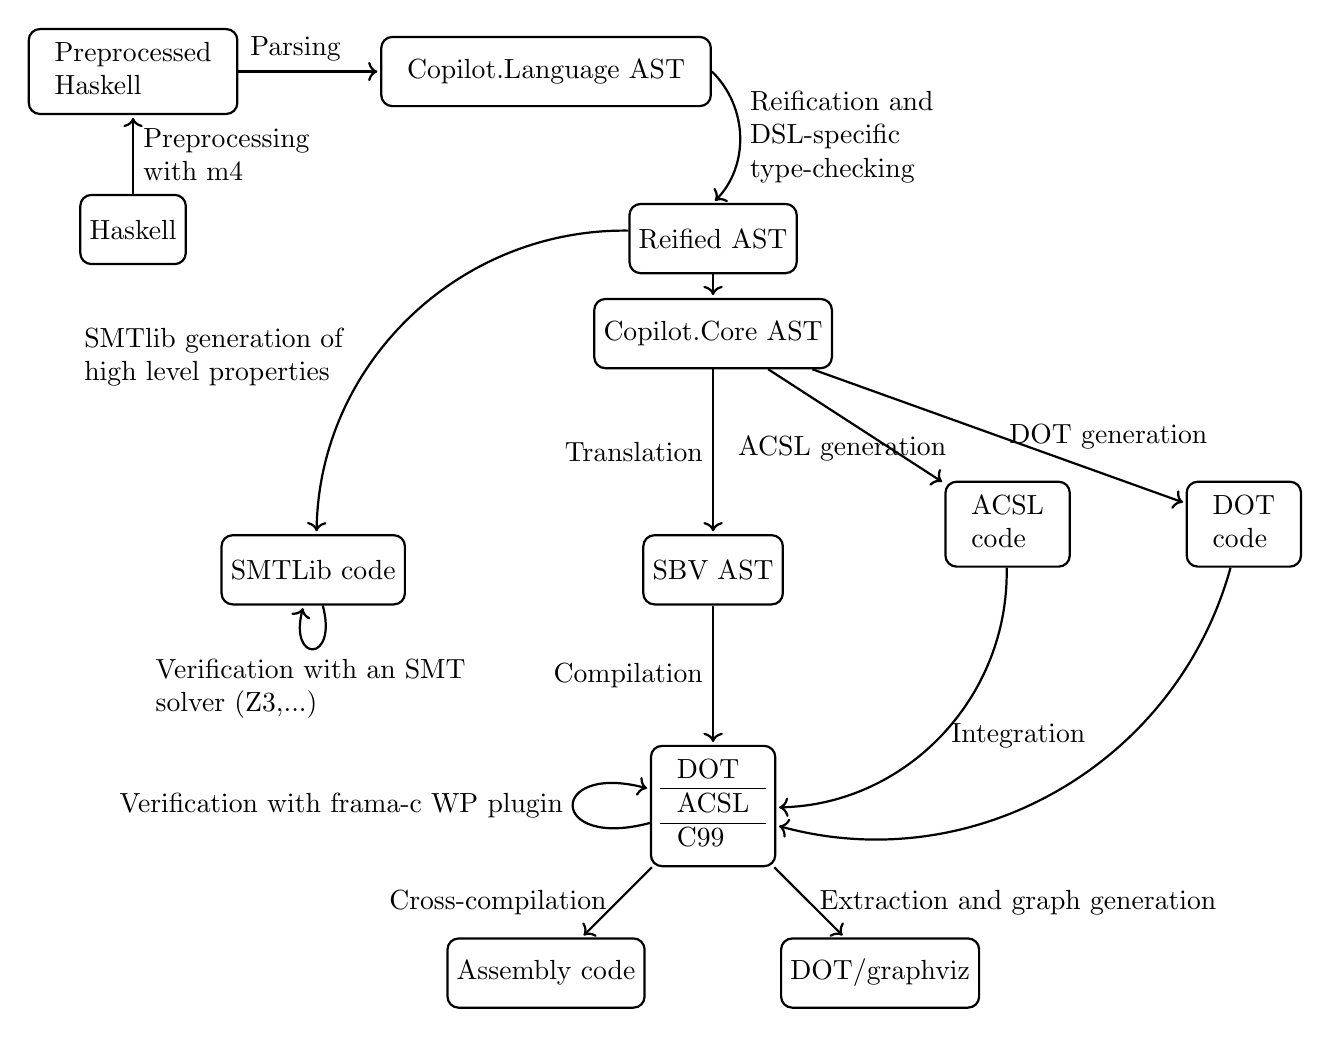
\begin{tikzpicture}[->, node distance=3cm, auto, shorten >=1pt, bend angle=45,
	thick]
	\tikzstyle{every state}=[rectangle, rounded corners]
	
	\node[state] (Lang) {%
		\begin{tabular}[b]{l}
		Copilot.Language AST
		\end{tabular}};
	
	\node[state] (M5) [left=1.8cm of Lang] {\begin{tabular}[b]{l}
		Preprocessed\\ Haskell
		\end{tabular}};
	\node[state] (M4) [below=1cm of M5] {Haskell};
	\node[state] (RR) [below right of=Lang] {Reified AST};
	\node[state] (Core) [below=0.3cm of RR] {Copilot.Core AST};
	
	
	\node[state] (ACSL) [below right= 2cm of Core] {\begin{tabular}[b]{l}
		ACSL\\ code
		\end{tabular}};
	\node[state] (DOTc) [right of=ACSL] {\begin{tabular}[b]{l}
		DOT\\ code
		\end{tabular}};
	\node[state] (SBV) [below of=Core] {SBV AST};
	\node[state] (C99S) [below of=SBV] {\begin{tabular}[b]{l}
		DOT\\ \hline ACSL\\ \hline C99
		\end{tabular}};
	\node[state] (DOT) [below right of=C99S] {DOT/graphviz};
	\node[state] (SMT) [left=3cm of SBV] {SMTLib code};
	\node[state] (ASM) [below left of= C99S] {Assembly code};
	
	
	\tikzstyle{every node}=[]
	
	
	\path %% (Libs) edge node {0,1,L} (Lang);
	%% edge node {1,1,R} (C)
	(Lang) edge [bend left, anchor=west, text width=2.5cm] node {Reification and DSL-specific type-checking} (RR)
	(RR) edge [anchor=west, text width=2.5cm] node {} (Core)
	%% edge node {0,1,L} (C)
	(M4) edge [text width=2.5cm, anchor = west] node {Preprocessing with m4} (M5)
	(M5) edge [text width=1.5cm] node {Parsing} (Lang)
	(Core) edge [anchor=east] node {Translation} (SBV)
	(ACSL) edge [bend left, anchor=west] node {Integration} (C99S)
	(DOTc) edge [bend left, anchor=east] node {} (C99S)
	(Core) edge [->, anchor=north, text width=3cm] node {ACSL generation} (ACSL)
	(Core) edge [->, anchor=west] node {DOT generation} (DOTc)
	(RR) edge [bend right, ->, anchor=north east,text width=4cm] node {SMTlib generation of high level properties} (SMT)
	(SMT) edge [loop below, ->, anchor=north,text width=4cm] node {Verification with an SMT solver (Z3,...)} (SMT)
	(C99S) edge [->, anchor=east] node {Cross-compilation} (ASM)
	(C99S) edge [loop left, ->, anchor=east] node {Verification with frama-c WP plugin} (C99S)
	(C99S) edge [->, anchor=west] node {Extraction and graph generation} (DOT)
	(SBV) edge [->,anchor=east] node {Compilation} (C99S);
	%% edge [bend left] node {Translation} (SBV)
	%% (Atom) edge [loop below] node {1,1,R} (D)
	%% edge node {0,1,R} (Libs)
	%% (SBV) edge [bend left] node {1,0,R} ();
	\end{tikzpicture}
	\caption{The new Copilot toolchain. The red arrows are the one to implement in the future.}
	\label{fig:WCVprocess}
\end{figure}
 
\addcontentsline{toc}{section}{References}
\bibliographystyle{alpha}
\bibliography{mybib}
}

\begin{appendices}
\documentclass[11pt]{article}

\usepackage[margin=2cm]{geometry}
\begin{document}
$$ \begin{array}{lcl}
\langle defs \rangle & ::= & (\langle def \rangle)^* \\
 & & \\
\langle ctype \rangle & ::= & \texttt{Bool} \\  
    & | & \texttt{Int8} \\
    & | & \texttt{Int16} \\ 
    & | & \texttt{Int32} \\
    & | & \texttt{Int64} \\
    & | & \texttt{Word8} \\ 
    & | & \texttt{Word16} \\
    & | & \texttt{Word32} \\
    & | & \texttt{Word64} \\
    & | & \texttt{Float} \\
    & | & \texttt{Double} \\
 & & \\
\langle def \rangle & ::= & (\langle id \rangle \texttt{::} \texttt{Stream } \langle ctype \rangle)? \langle id \rangle \texttt{=}\langle spec \rangle \\
 & & \\
\langle id \rangle & ::= & (\texttt{a}-\texttt{z})(\texttt{a}-\texttt{z}|\texttt{A}-\texttt{Z}|\texttt{0}-\texttt{9}|\_|\texttt{-}|\texttt{'})^* \\
 & & \\
%\mbox{\emph{string}} & ::= & \texttt{"}(\emph{printableChar})^*\texttt{"} \\
%    & | & \mbox{\emph{string} \texttt{++} \emph{string}} \\ 
%    & | & \texttt{[]} \\ 
%    & | & \mbox{\texttt{'}\emph{printableChar}\texttt{'} \texttt{:} \emph{string}} \\ 
 & & \\
\langle string \rangle & ::= & \texttt{"}(\texttt{a}-\texttt{z}|\texttt{A}-\texttt{Z})(\texttt{a}-\texttt{z}|\texttt{A}-\texttt{Z}|\texttt{\_}|\texttt{0}-\texttt{9})_{\leq 30}^*\texttt{"} \\
 & & \\
\langle stream \rangle & ::= & \langle valueList \rangle \texttt{++} \langle stream \rangle \\
    & | & \langle funStream \rangle \\ 
& & \\ 
\langle valueList \rangle & ::= & [(\langle vbool \rangle)_,^*] \\
    & | & [(\langle vint \rangle)_,^*] \\ 
    & | & [(\langle vfloat \rangle)_,^*] \\ 
 & & \\ 
\langle vbool \rangle & ::= & \texttt{true} \\
    & | & \texttt{false} \\
 & & \\
\langle vint \rangle & ::= & [\texttt{+}|\texttt{-}](\texttt{0}-\texttt{9})^+ \\
 & & \\
\langle vfloat \rangle & ::= & \langle vint \rangle .(\texttt{0}-\texttt{9})^+ \\
 & & \\
\langle funStream \rangle & ::= & \langle externV \rangle~ \langle string \rangle~ \langle contextV \rangle \\
    & | & \texttt{label} ~ \langle string \rangle ~ \langle funStream \rangle \\
    & | & \texttt{externFun} ~ \langle string \rangle ~ \langle argList \rangle ~ \langle contextF \rangle \\
    & | & \langle externA \rangle ~ \langle string \rangle ~ \langle stream \rangle ~ \langle int \rangle ~ \langle contextA \rangle \\
    & | & \langle op1 \rangle ~ \langle  funStream \rangle \\
    & | & \langle funStream \rangle ~ \langle  op2Infix \rangle ~ \langle funStream \rangle \\
    & | & \langle op3 \rangle ~ \langle funStream \rangle ~ \langle funStream \rangle ~ \langle funStream \rangle \\
    & | & \langle dropStream \rangle \\
 & & \\


\end{array} $$
$$ \begin{array}{lcl}
 \langle externV \rangle & ::= &  \mbox{\texttt{extern}} \\
    & | & \mbox{\texttt{externB}} \\
    & | & \mbox{\texttt{externI8}} \\
    & | & \mbox{\texttt{externI16}} \\
    & | & \mbox{\texttt{externI32}} \\
    & | & \mbox{\texttt{externI64}} \\
    & | & \mbox{\texttt{externW8}} \\
    & | & \mbox{\texttt{externW16}} \\
    & | & \mbox{\texttt{externW32}} \\
    & | & \mbox{\texttt{externW64}} \\
    & | & \mbox{\texttt{externF}} \\
    & | & \mbox{\texttt{externD}} \\
 & & \\
 \langle externA \rangle & ::= &  \mbox{\texttt{externArray}} \\
    & | & \mbox{\texttt{externArrayB}} \\
    & | & \mbox{\texttt{externArrayI8}} \\
    & | & \mbox{\texttt{externArrayI16}} \\
    & | & \mbox{\texttt{externArrayI32}} \\
    & | & \mbox{\texttt{externArrayI64}} \\
    & | & \mbox{\texttt{externArrayW8}} \\
    & | & \mbox{\texttt{externArrayW16}} \\
    & | & \mbox{\texttt{externArrayW32}} \\
    & | & \mbox{\texttt{externArrayW64}} \\
    & | & \mbox{\texttt{externArrayF}} \\
    & | & \mbox{\texttt{externArrayD}} \\

 & & \\
 \langle contextV \rangle & ::= &  \mbox{\texttt{Nothing}} \\
    & | & \mbox{\texttt{Just}} ~ \langle stream \rangle \\
 & & \\
 \langle contextF \rangle & ::= &  \mbox{\texttt{Nothing}} \\
    & | & \mbox{\texttt{Just}} ~ \langle stream \rangle \\
 & & \\
\langle contextA \rangle & ::= &  \mbox{\texttt{Nothing}} \\
    & | & \texttt{Just } [(\langle valueList \rangle)_,^*]  \\

 & & \\
\langle argList \rangle & ::= &  [(\mbox{\texttt{Arg }} \langle stream \rangle)_,^*]  \\
    & | & \texttt{[]} \\
    & | & (\texttt{Arg } \langle stream \rangle)\texttt{:} \langle argList \rangle \\
 & & \\
\end{array} $$
$$ \begin{array}{lcl}
\langle dropStream \rangle & ::= & \langle id \rangle \\
    & | & \mbox{\texttt{constant}} ~ \langle value \rangle \\
    & | & \mbox{\texttt{drop}} ~ \langle int \rangle~\langle stream \rangle \\
 & & \\


\langle op1\rangle & ::= & \texttt{not} ~|~ \texttt{abs} ~|~ \texttt{signum}~|~ \texttt{complement}\\
&|&\texttt{recip}~|~ \texttt{exp}~|~ \texttt{sqrt}\\
&|& \texttt{log}~|~ \texttt{sin}~|~ \texttt{cos}~|~ \texttt{tan}\\
&|& \texttt{asin}~|~ \texttt{acos}~|~ \texttt{atan}\\
&|& \texttt{sinh}~|~ \texttt{cosh}~|~ \texttt{tanh}\\
&|& \texttt{asinh}~|~ \texttt{acosh}~|~ \texttt{atanh}\\
&|& \texttt{cast}~|~ \texttt{unsafeCast}\\
 & & \\
\langle op2Infix \rangle & ::= &  \texttt{+}~|~\texttt{-}~|~\texttt{*}~|~ \texttt{`mod`}~|~\texttt{`div`} \\
    & | & \texttt{/}~|~\texttt{**}~|~\texttt{`logBase`} \\
    & | & \texttt{<}~|~\texttt{<=}~|~\texttt{==}~|~\texttt{/=}~|~\texttt{>=}~|~\texttt{>} \\
    & | & \texttt{||}~|~ \texttt{\&\&}~|~ \texttt{`xor`}~|~ \texttt{==>} \\
    & | & \texttt{.\&.}~|~ \texttt{.|.}~|~\texttt{.\textasciicircum.}~|~ \texttt{.>>.}~|~ \texttt{.<<.}  \\
 & & \\
\langle op3 \rangle & ::= & \texttt{mux} \\
 & & \\
%\mbox{\emph{printableChar}} & ::= & \texttt{!}|\texttt{ }|\texttt{\textbackslash "}|\texttt{\#}|\texttt{\$}|\texttt{\%}|\texttt{\&}|\texttt{'}|\texttt{(}|\texttt{)}|\texttt{*}|\texttt{+}|\texttt{,}|\texttt{-} \\
%& | & \texttt{.}|\texttt{/}|\texttt{0}-\texttt{9}|\texttt{:}|\texttt{;}|\texttt{<}|\texttt{=}|\texttt{>}|\texttt{?}|\texttt{@}|\texttt{A}-\texttt{Z} \\
%& | & \texttt{[}|\texttt{\textbackslash}|\texttt{]}|\texttt{\textasciicircum}|\texttt{\_}|\texttt{`}|\texttt{a}-\texttt{z}|\texttt{\{}|\texttt{|}|\texttt{\}}|\texttt{\textasciitilde} \\

\end{array} $$

\end{document}

\documentclass[11pt]{article}

\usepackage{bcprules}

\begin{document}

\infrule[stringConst]
    {s \mbox{ is a } \langle string \rangle \mbox{ token}} 
    {\Gamma \vdash s : \texttt{String}}
\infrule[inst]
    {\tau \in{ \mbox{inst}(\Gamma (s))}} 
    {\Gamma \vdash s : \tau}
\infrule[arg]
    {\Gamma \vdash s : \texttt{Stream } \tau} 
    {\Gamma \vdash \texttt{Arg } s : \texttt{Arg}}
%\infrule[argL]
%    {} 
%    {\Gamma \vdash \texttt{[]} : \texttt{Arg}}
%\infrule[argLCons]
%    {\Gamma \vdash h : \texttt{Arg} \andalso \Gamma \vdash t : \texttt{[Arg]}} 
%    {\Gamma \vdash h\texttt{:}t : \texttt{[Arg]}}
%\infrule[argL2]
%    {\Gamma \vdash x_1, ..., x_n : \texttt{Arg}} 
%    {\Gamma \vdash \texttt{[}x_1 \texttt{,} ... \texttt{,} x_n \texttt{]} : \texttt{[Arg]}}
\infrule[valConst]
    {\Gamma \vdash x : \tau} 
    {\Gamma  \vdash {\texttt{constant } x : \texttt{Stream } \tau }}
\infrule[drop]
    {\Gamma \vdash i : \texttt{Integer} \andalso \Gamma \vdash x :  \texttt{Stream } \tau} 
    {\Gamma  \vdash {\texttt{drop } i~x : \texttt{Stream } \tau }}
\infrule[Append] 
    {\Gamma \vdash ls : [a] \andalso \Gamma \vdash s : \mbox{Spec } a} 
    {\Gamma \vdash ls ++ s : \mbox{Spec } a}


\infrule[label]
    {\Gamma \vdash s : \texttt{String} \andalso \Gamma \vdash x : \texttt{Stream } \tau} 
    {\Gamma  \vdash {\texttt{label } s~x : \texttt{Stream } \tau }}

\infrule[ext]
    {\Gamma \vdash s : \texttt{String} \andalso \Gamma \vdash x : \texttt{Stream } \tau} 
    {\Gamma  \vdash {\texttt{extern } s~x : \texttt{Stream } \tau }}
\infrule[extB]
    {\Gamma \vdash s : \texttt{String} \andalso \Gamma \vdash x : \texttt{Stream Bool}} 
    {\Gamma  \vdash {\texttt{externB } s~x : \texttt{Stream Bool}}}
\infrule[extI8]
    {\Gamma \vdash s : \texttt{String} \andalso \Gamma \vdash x : \texttt{Stream Int8}} 
    {\Gamma  \vdash {\texttt{externI8 } s~x : \texttt{Stream Int8}}}
\infrule[extI16]
    {\Gamma \vdash s : \texttt{String} \andalso \Gamma \vdash x : \texttt{Stream Int16}} 
    {\Gamma  \vdash {\texttt{externI16 } s~x : \texttt{Stream Int16}}}
\infrule[extI32]
    {\Gamma \vdash s : \texttt{String} \andalso \Gamma \vdash x : \texttt{Stream Int32}} 
    {\Gamma  \vdash {\texttt{externI32 } s~x : \texttt{Stream Int32}}}
\infrule[extI64]
    {\Gamma \vdash s : \texttt{String} \andalso \Gamma \vdash x : \texttt{Stream Int64}} 
    {\Gamma  \vdash {\texttt{externI64 } s~x : \texttt{Stream Int64}}}
\infrule[extW8]
    {\Gamma \vdash s : \texttt{String} \andalso \Gamma \vdash x : \texttt{Stream Word8}} 
    {\Gamma  \vdash {\texttt{externW8 } s~x : \texttt{Stream Word8}}}
\infrule[extW16]
    {\Gamma \vdash s : \texttt{String} \andalso \Gamma \vdash x : \texttt{Stream Word16}} 
    {\Gamma  \vdash {\texttt{externW16 } s~x : \texttt{Stream Word16}}}
\infrule[extW32]
    {\Gamma \vdash s : \texttt{String} \andalso \Gamma \vdash x : \texttt{Stream Word32}} 
    {\Gamma  \vdash {\texttt{externW32 } s~x : \texttt{Stream Word32}}}
\infrule[extW64]
    {\Gamma \vdash s : \texttt{String} \andalso \Gamma \vdash x : \texttt{Stream Word64}} 
    {\Gamma  \vdash {\texttt{externW64 } s~x : \texttt{Stream Word64}}}
\infrule[extFloat]
    {\Gamma \vdash s : \texttt{String} \andalso \Gamma \vdash x : \texttt{Stream Float}} 
    {\Gamma  \vdash {\texttt{externF } s~x : \texttt{Stream Float}}}
\infrule[extDouble]
    {\Gamma \vdash s : \texttt{String} \andalso \Gamma \vdash x : \texttt{Stream Double}} 
    {\Gamma  \vdash {\texttt{externD } s~x : \texttt{Stream Double}}}


\infrule[extFun]
    {\Gamma \vdash s : \texttt{String} \andalso \Gamma \vdash a : \texttt{[Arg]} \andalso \Gamma \vdash x : \texttt{Stream } \tau} 
    {\Gamma  \vdash {\texttt{externFun } s~a~x : \texttt{Stream } \tau}}

\infrule[extA]
    {\Gamma \vdash s : \texttt{String} \andalso \Gamma \vdash i : \texttt{Integral } \tau_1\Rightarrow \texttt{Stream } \tau_1 \andalso \Gamma \vdash m : \texttt{Integer} \andalso \Gamma \vdash x :  \texttt{[[} \tau \texttt{]]}} 
    {\Gamma  \vdash {\texttt{externArray } s~i~m~x : \texttt{Stream } \tau }}

\infrule[extAB]
    {\Gamma \vdash s : \texttt{String} \andalso \Gamma \vdash i : \texttt{Integral } \tau_1\Rightarrow \texttt{Stream } \tau_1 \andalso \Gamma \vdash m : \texttt{Integer} \andalso \Gamma \vdash x :  \texttt{[[Bool]]}} 
    {\Gamma  \vdash {\texttt{externArrayB } s~i~m~x : \texttt{Stream Bool}}}


\infrule[extAI8]
    {\Gamma \vdash s : \texttt{String} \andalso \Gamma \vdash i : \texttt{Integral } \tau_1\Rightarrow \texttt{Stream } \tau_1 \andalso \Gamma \vdash m : \texttt{Integer} \andalso \Gamma \vdash x :  \texttt{[[Int8]]}} 
    {\Gamma  \vdash {\texttt{externArrayI8 } s~i~m~x : \texttt{Stream Int8}}}

\infrule[extAI16]
    {\Gamma \vdash s : \texttt{String} \andalso \Gamma \vdash i : \texttt{Integral } \tau_1\Rightarrow \texttt{Stream } \tau_1 \andalso \Gamma \vdash m : \texttt{Integer} \andalso \Gamma \vdash x :  \texttt{[[Int16]]}} 
    {\Gamma  \vdash {\texttt{externArrayI16 } s~i~m~x : \texttt{Stream Int16}}}
\infrule[extAI32]
    {\Gamma \vdash s : \texttt{String} \andalso \Gamma \vdash i : \texttt{Integral } \tau_1\Rightarrow \texttt{Stream } \tau_1 \andalso \Gamma \vdash m : \texttt{Integer} \andalso \Gamma \vdash x :  \texttt{[[Int32]]}} 
    {\Gamma  \vdash {\texttt{externArrayI32 } s~i~m~x : \texttt{Stream Int32}}}
\infrule[extAI64]
    {\Gamma \vdash s : \texttt{String} \andalso \Gamma \vdash i : \texttt{Integral } \tau_1\Rightarrow \texttt{Stream } \tau_1 \andalso \Gamma \vdash m : \texttt{Integer} \andalso \Gamma \vdash x :  \texttt{[[Int64]]}} 
    {\Gamma  \vdash {\texttt{externArrayI64 } s~i~m~x : \texttt{Stream Int64}}}

\infrule[extAW8]
    {\Gamma \vdash s : \texttt{String} \andalso \Gamma \vdash i : \texttt{Integral } \tau_1\Rightarrow \texttt{Stream } \tau_1 \andalso \Gamma \vdash m : \texttt{Integer} \andalso \Gamma \vdash x :  \texttt{[[Word8]]}} 
    {\Gamma  \vdash {\texttt{externArrayW8 } s~i~m~x : \texttt{Stream Word8}}}
\infrule[extAW16]
    {\Gamma \vdash s : \texttt{String} \andalso \Gamma \vdash i : \texttt{Integral } \tau_1\Rightarrow \texttt{Stream } \tau_1 \andalso \Gamma \vdash m : \texttt{Integer} \andalso \Gamma \vdash x :  \texttt{[[Word16]]}} 
    {\Gamma  \vdash {\texttt{externArrayW16 } s~i~m~x : \texttt{Stream Word16}}}
\infrule[extAW32]
    {\Gamma \vdash s : \texttt{String} \andalso \Gamma \vdash i : \texttt{Integral } \tau_1\Rightarrow \texttt{Stream } \tau_1 \andalso \Gamma \vdash m : \texttt{Integer} \andalso \Gamma \vdash x :  \texttt{[[Word32]]}} 
    {\Gamma  \vdash {\texttt{externArrayW32 } s~i~m~x : \texttt{Stream Word32}}}
\infrule[extAW64]
    {\Gamma \vdash s : \texttt{String} \andalso \Gamma \vdash i : \texttt{Integral } \tau_1\Rightarrow \texttt{Stream } \tau_1 \andalso \Gamma \vdash m : \texttt{Integer} \andalso \Gamma \vdash x :  \texttt{[[Word64]]}} 
    {\Gamma  \vdash {\texttt{externArrayW64 } s~i~m~x : \texttt{Stream Word64}}}
\infrule[extAFloat]
    {\Gamma \vdash s : \texttt{String} \andalso \Gamma \vdash i : \texttt{Integral } \tau_1\Rightarrow \texttt{Stream } \tau_1 \andalso \Gamma \vdash m : \texttt{Integer} \andalso \Gamma \vdash x :  \texttt{[[Float]]}} 
    {\Gamma  \vdash {\texttt{externArrayF } s~i~m~x : \texttt{Stream Float}}}
\infrule[extADouble]
    {\Gamma \vdash s : \texttt{String} \andalso \Gamma \vdash i : \texttt{Integral } \tau_1\Rightarrow \texttt{Stream } \tau_1 \andalso \Gamma \vdash m : \texttt{Integer} \andalso \Gamma \vdash x :  \texttt{[[Double]]}} 
    {\Gamma  \vdash {\texttt{externArrayD } s~i~m~x : \texttt{Stream Double}}}


\infrule[op1Bool]
    {\Gamma \vdash x : \texttt{Stream Bool} \andalso op \in \{ \texttt{not} \}} 
    {\Gamma  \vdash {op~x : \texttt{Stream Bool}}}


\infrule[op1Bitwise]
    {\Gamma \vdash x :  \texttt{Bits } \tau \Rightarrow \texttt{Stream } \tau \andalso op \in \{\texttt{complement} \}} 
    {\Gamma  \vdash {op~x : \texttt{Stream } \tau}}

\infrule[op1Num]
    {\Gamma \vdash x :  \texttt{Integral } \tau \Rightarrow \texttt{Stream } \tau \andalso op \in \{ \texttt{abs},\texttt{signum} \}} 
    {\Gamma  \vdash {op~x : \texttt{Stream } \tau}}


\infrule[op2Bool]
    {\Gamma \vdash x : \texttt{Stream Bool} \andalso \Gamma \vdash y : \texttt{Stream Bool} \andalso op \in \{ \texttt{||},\texttt{\&\&},\texttt{`xor`},\texttt{==>} \}} 
    {\Gamma  \vdash {op~x~y : \texttt{Stream Bool}}}



\infrule[op2Integral]
    {\Gamma \vdash x :  \texttt{Integral } \tau \Rightarrow\texttt{Stream }  \tau \andalso \Gamma \vdash y : \texttt{Integral } \tau  \Rightarrow \texttt{Stream }  \tau \andalso op \in \{ \texttt{`mod`}, \texttt{`div`} \}} 
    {\Gamma  \vdash {op~x~y : \texttt{Stream } \tau}}



\infrule[op2Fractionnal]
    {\Gamma \vdash x :  \texttt{Fractionnal } \tau \Rightarrow\texttt{Stream }  \tau \andalso \Gamma \vdash y : \texttt{Fractionnal } \tau  \Rightarrow \texttt{Stream }  \tau \andalso op \in \{ \texttt{/} \}} 
    {\Gamma  \vdash {op~x~y : \texttt{Stream } \tau}}

\infrule[op2Floating]
    {\Gamma \vdash x :  \texttt{Floating } \tau \Rightarrow\texttt{Stream }  \tau \andalso \Gamma \vdash y : \texttt{Floating } \tau  \Rightarrow \texttt{Stream }  \tau \andalso op \in \{ \texttt{**},\texttt{`logBase`} \}} 
    {\Gamma  \vdash {op~x~y : \texttt{Stream } \tau}}

\infrule[op2Num]
    {\Gamma \vdash x :  \texttt{Num } \tau \Rightarrow\texttt{Stream }  \tau \andalso \Gamma \vdash y : \texttt{Num } \tau  \Rightarrow \texttt{Stream }  \tau \andalso op \in \{ \texttt{+}, \texttt{-}, \texttt{*} \}} 
    {\Gamma  \vdash {op~x~y : \texttt{Stream } \tau}}

\infrule[op2Eq]
    {\Gamma \vdash x :  \texttt{Eq } \tau \Rightarrow\texttt{Stream }  \tau \andalso \Gamma \vdash y : \texttt{Eq } \tau  \Rightarrow \texttt{Stream }  \tau \andalso op \in \{ \texttt{==}, \texttt{/=} \}} 
    {\Gamma  \vdash {op~x~y : \texttt{Stream } \tau}}

\infrule[op2Ord]
    {\Gamma \vdash x :  \texttt{Ord } \tau \Rightarrow\texttt{Stream }  \tau \andalso \Gamma \vdash y : \texttt{Ord } \tau  \Rightarrow \texttt{Stream }  \tau \andalso op \in \{ \texttt{<},\texttt{<=}, \texttt{>=}, \texttt{>}\}} 
    {\Gamma  \vdash {op~x~y : \texttt{Stream } \tau}}


\infrule[op2Bitwise]
    {\Gamma \vdash x :  \texttt{Bits } \tau \Rightarrow\texttt{Stream }  \tau \andalso \Gamma \vdash y : \texttt{Bits } \tau  \Rightarrow \texttt{Stream }  \tau \andalso op \in \{ \texttt{.\&.},\texttt{.|.}, \texttt{.\textasciicircum.}\}} 
    {\Gamma  \vdash {op~x~y : \texttt{Stream } \tau}}

\infrule[op2BwShift]
    {\Gamma \vdash x :  \texttt{Bits } \tau \Rightarrow\texttt{Stream }  \tau \andalso \Gamma \vdash y : \texttt{Integral } \tau_1  \Rightarrow \texttt{Stream }  \tau_1 \andalso op \in \{ \texttt{.>>.},\texttt{.<<.}\}} 
    {\Gamma  \vdash {op~x~y : \texttt{Stream } \tau}}

\infrule[op3]
    {\Gamma \vdash x : \texttt{Stream Bool} \andalso \Gamma \vdash y : \texttt{Stream } \tau \andalso \Gamma \vdash z : \texttt{Stream } \tau \andalso op \in \{ \texttt{mux} \}} 
    {\Gamma  \vdash {op~x~y~z : \texttt{Stream } \tau}}

\end{document}

\end{appendices}
\end{document}

